\documentclass{beamer}
\usetheme{Warsaw}
\usecolortheme{crane}
\setbeamercolor{structure}{fg=goldenrod}

\setbeamertemplate{navigation symbols}{}

\usepackage{listings}
\definecolor{codegreen}{rgb}{0,0.6,0}
\definecolor{codegray}{rgb}{0,0,0}
\definecolor{codepurple}{rgb}{0.58,0,0.82}
\definecolor{backcolour}{rgb}{0.95,0.95,0.92}

\lstdefinestyle{mystyle}{
    backgroundcolor=\color{backcolour},
    commentstyle=\color{codegreen},
    keywordstyle=\color{magenta},
    numberstyle=\tiny\color{codegray},
    stringstyle=\color{codepurple},
    basicstyle=\ttfamily\small,
    breakatwhitespace=false,
    breaklines=true,
    captionpos=b,
    keepspaces=true,
    numbers=left,
    numbersep=5pt,
    showspaces=false,
    showstringspaces=false,
    showtabs=false,
    tabsize=2
}

\lstset{style=mystyle}
\lstset{language=Python}

\lstset{
literate=
{á}{{\'a}}1 {é}{{\'e}}1 {í}{{\'i}}1 {ó}{{\'o}}1 {ú}{{\'u}}1
{à}{{\`a}}1 {è}{{\`e}}1 {ì}{{\`i}}1 {ò}{{\`o}}1 {ù}{{\`u}}1
{€}{{\euro}}1 {ê}{{\^e}}1 {â}{{\^a}}1 {ô}{{\^o}}1
}

\setbeamertemplate{headline}{} 

\begin{document}
\title{Diverses méthodes d'intégration}
\author{SAMER Ahmed Wahid}

\begin{frame}

\titlepage
\end{frame}

\begin{frame}

\frametitle{Sommaire}
\tableofcontents
\end{frame}
\setbeamertemplate{navigation symbols}{}
\usenavigationsymbolstemplate{}

\section{Introduction}
\setbeamertemplate{headline}{} 
\begin{frame}
\frametitle{Introduction}

\begin{center}
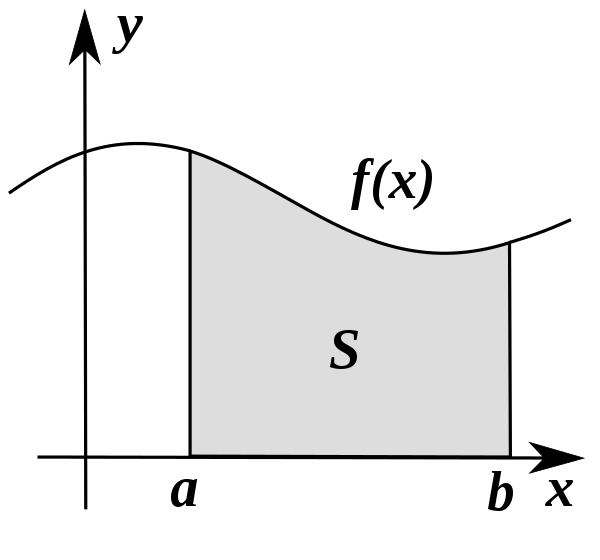
\includegraphics[scale=0.2]{600px-Integral_as_region_under_curve.svg.png} \\
{\displaystyle \textstyle S=\int _{a}^{b}f(x)\,\mathrm {d} x}

\end{center}

\end{frame}

\begin{frame}
\frametitle{Introduction}

\begin{center}
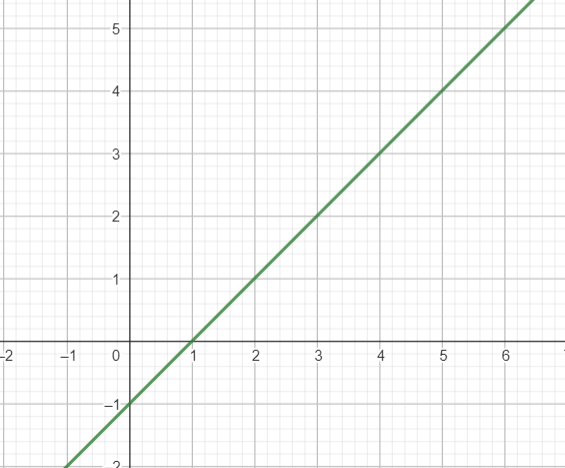
\includegraphics[scale=0.7]{f(x)=x-1.png} 
\[ f(x) = x - 1 \]
\end{center}

\end{frame}

\begin{frame}
\frametitle{Introduction}

\begin{center}
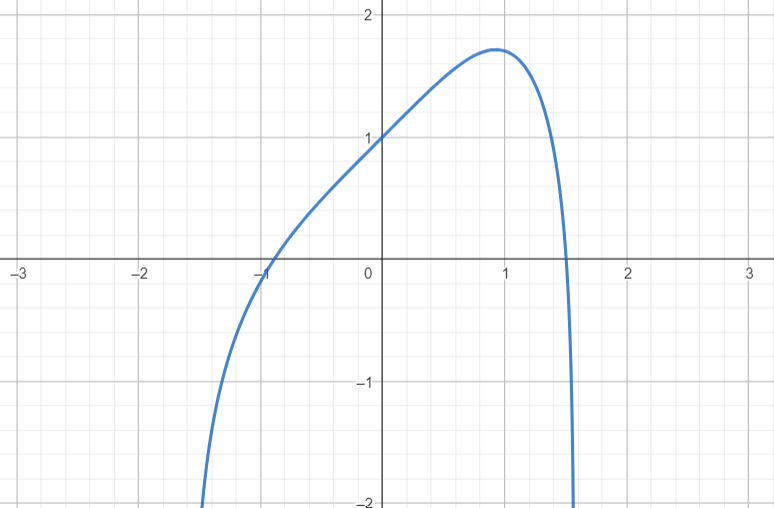
\includegraphics[scale=0.7]{g(x)=e(sin(x))+ln(cos(x)).png} 
\[ g(x) = e^{\sin(x)} + \ln(\cos(x)) \]
\end{center}

\end{frame}

\section{La Méthode de Simpson}
\setbeamertemplate{headline}{} 
\begin{frame}
\frametitle{La Méthode de Simpson}

\begin{block}{Formule de Simpson}
La formule de Simpson pour approximer l'intégrale sur un intervalle $[a, b]$ est donnée par :
\[ \int_a^b f(x) \, dx \approx \frac{h}{3} \left[ f(a) + 4f\left(\frac{a+b}{2}\right) + f(b) \right] \]
où $h = \frac{b - a}{2}$ est la taille de l'intervalle.
\end{block}
\end{frame}

\begin{frame}
\frametitle{La Méthode de Simpson}
\begin{center}
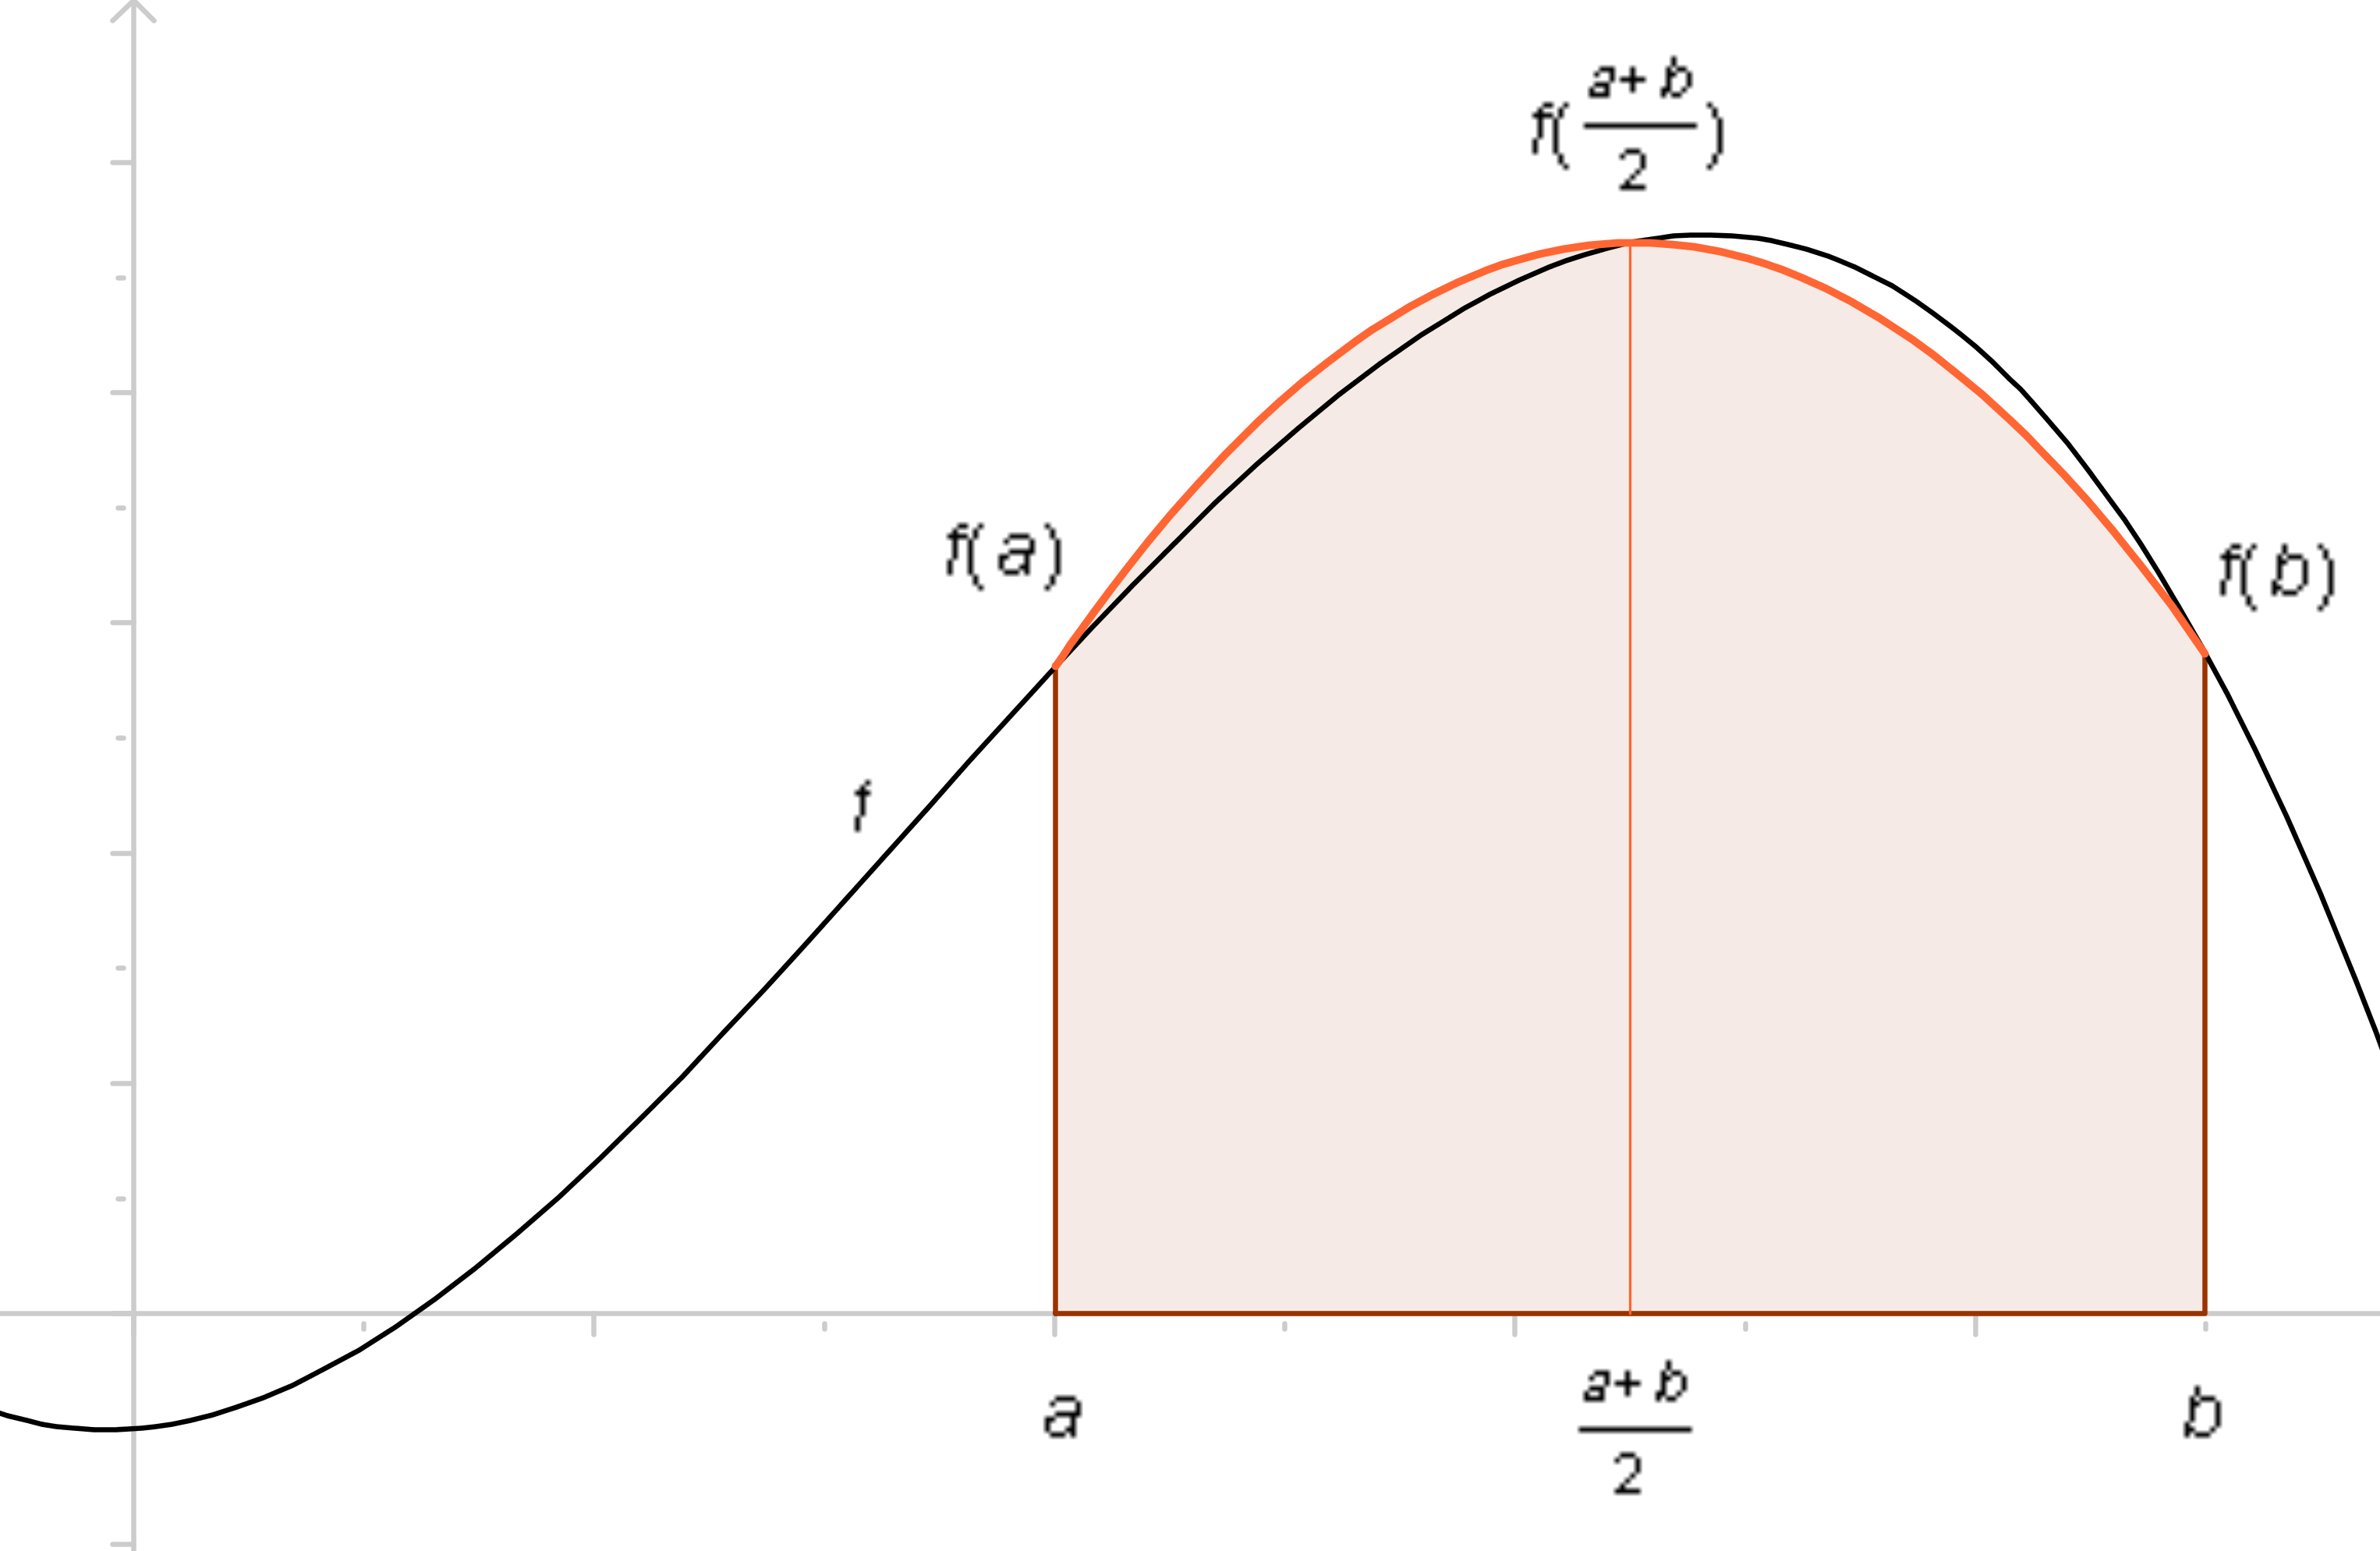
\includegraphics[scale=0.15]{Simpson_rule.png} \\ La courbe rouge représente le polynôme d'approximation P(x).
\end{center}
\end{frame}

\begin{frame}[fragile]
\frametitle{La Méthode Simpson}
\begin{lstlisting}[language=Python]
def simpson(f, a, b, n):
    if n % 2 != 0:
        raise ValueError("Le nombre n'est pas pair.")
    
    h = (b - a) / n
    x = [a + i * h for i in range(n+1)]
    y = [f(x[i]) for i in range(n+1)]
    
    integral = y[0] + y[-1] 
    
    for i in range(1, n, 2):
        integral += 4 * y[i]
    
    for i in range(2, n-1, 2):
        integral += 2 * y[i]
    
    integral *= h / 3
    return integral
\end{lstlisting}
\end{frame}


\section{La Méthode d'Euler}
\begin{frame}
\frametitle{La Méthode d'Euler}

\begin{block}{Formule de la Méthode d'Euler}
La formule de la méthode d'Euler pour résoudre une EDO du premier ordre de la forme $y'(t) = f(t, y(t))$ est donnée par :
\[ y_{n+1} = y_n + hf(t_n, y_n) \]
où $h$ est la taille du pas de temps, $y_n$ est l'approximation de la solution à l'instant $t_n$, et $f(t_n, y_n)$ est la pente de la solution à cet instant.
\end{block}


\end{frame}

\begin{frame}
\frametitle{La Méthode d'Euler}
\begin{center}
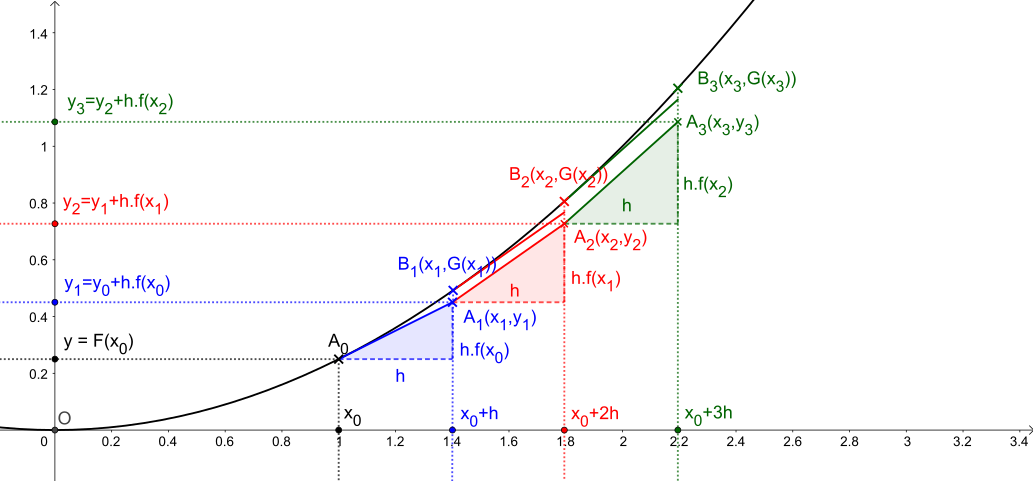
\includegraphics[scale=0.3]{Integration_x_div_2.png}\\
Illustration de la méthode d'Euler
\end{center}
\end{frame}
 
\begin{frame}[fragile]
\frametitle{La Méthode d'Euler}
\begin{lstlisting}[language=Python]
def euler(f, x0, y0, h, n):

    x_v = [x0] 
    y_v = [y0]  
    
    for i in range(1, n+1):
        x = x0 + i * h
        y = y_v[-1] + h * f(x_v[-1], y_v[-1])
        x_v.append(x)
        y_v.append(y)
    
    return x_v, y_v
\end{lstlisting}
\end{frame}

\section{Conclusion}

\begin{frame}
\frametitle{Conclusion}
Calcul de l'intégrale de $f(x) = x - 1$ sur l'intervalle $[0, 1]$ :

\begin{align*}
\int_{0}^{1} (x - 1) \, dx &= \left[\frac{x^2}{2} - x\right]_{0}^{1} \\
&= \left(\frac{1^2}{2} - 1\right) - \left(\frac{0^2}{2} - 0\right) \\
&= \frac{1}{2} - 1 \\
&= -\frac{1}{2}
\end{align*}
\end{frame}

\begin{frame}
\frametitle{Conclusion}
Pour $f(x)$ :
\begin{itemize}
    \item Méthode de Gauss : $-0.5$
    \item Méthode de Simpson : $-0.49999999999999983$
    \item Méthode de Monte Carlo : $-0.5065533679174838$
    \item Méthode des trapèzes : $-0.5000000000000001$
    \item Méthode des rectangles : $-0.5005000000000001$
\end{itemize}
\end{frame}

\begin{frame}
\frametitle{Conclusion}


\[
\int_{0}^{1} \left e^{\sin(x)} + \ln(\cos(x))\right \, dx
\]
\\
\begin{center}
Cette intégrale n'a pas de solution analytique simple.
\end{center}
\end{frame}

\begin{frame}
\frametitle{Conclusion}
Pour $g(x)$ :
\begin{itemize}
    \item Méthode de Gauss : $1.44433143939722$
    \item Méthode de Simpson : $1.4443314393971325$
    \item Méthode de Monte Carlo : $1.4503592007838038$
    \item Méthode des trapèzes : $1.444331330728321$
    \item Méthode des rectangles : $1.4439792555511564$
\end{itemize}
\end{frame}


\section{Remerciements}
\begin{frame}
\frametitle{Remerciements}
\begin{block}{}
\begin{center}
\Huge Merci de votre attention !
\end{center}
\end{block}
\end{frame}


\section{Références}
\begin{frame}
\frametitle{Références}
\begin{itemize}
\\
\item wikipedia (Wolfgang Dvorak), https://fr.wikipedia.org/wiki/M\%C3\%A9thode_de_Simpson, 8.03.2006.

\item wikipedia (Kelam), https://fr.wikipedia.org/wiki/M\%C3\%A9thode_d\%27Euler, 13 avril 2021.

\item wikiversity, https://fr.wikiversity.org/wiki/Approche_th\%C3\%A9orique_du_calcul_int\%C3\%A9gral.

\item SAMER et lechani, Geogebra, f(x) et g(x), 20/04/2024
\end{itemize}
\end{frame}

\end{document}
